\section*{Author's Note --- Advice for reading}
\label{sec:authors-note}
\addcontentsline{toc}{section}{Author's Note --- Advice for reading}

\noindent A short note from me (Florian Krebs), placed up front
because \emph{how} you read this paper matters as much as
\emph{what} is in it. This is a position paper, not a survey: the
contribution is a stance, that FAIR is insufficient for
LLM-assisted scholarly writing in its current form and that the
eight integrated practices of \S\ref{sec:eight} are the minimum
discipline an honest author can adopt today. The paper defends that
stance; a reader who comes looking for a survey will find an
argument. F(AI)\textsuperscript{2}R is a snapshot of a moving
target --- model capabilities, disclosure norms, and licensing
postures will move under us; the version manifest in
\texttt{doc/provenance.ttl} is the receipt that lets a future
reader date what we committed to.

\paragraph{The partition the cooperation makes visible.}
A second-order observation, recorded for the recursive case study
(\S\ref{sec:evolution}). Cooperative writing with an LLM, as
practised here, partitions cleanly: the human does the abstraction,
the logical reasoning, and the choice of the next step; the model
takes those decisions and turns them into readable prose.
\emph{The human does the deciding, the model does the drafting, and
naming the partition is itself a methodological act.} The pattern
this paper describes is designed to make that partition legible
from outside the session --- in the prompts, in the transcripts,
and in the graph. The human-side contribution is structural and
corrective (deciding the position, abstracting the eight-practice
integration, catching drift, staking reputation under a published
name); the model-side contribution is volume and second-order
pattern-matching (drafting at scale, cross-referencing, keeping
graph and manuscript in sync). Human interventions are rare in
volume but high in leverage
(Figure~\ref{fig:contribution-histogram}); model outputs are long
and constant
but low in irreversibility.

% Coupling rule: prose-craft / abstracting partition with accelerator-vs-
% blender outcomes. Visualises the second-order finding in the Author's
% Note (sec:authors-note, "What surprised me about the cooperation").
% Loaded by paper/sections/authors-note.tex via \input.
\begin{figure}[!t]
\centering
\begin{tikzpicture}[
  node distance=0pt,
  every node/.style={font=\sffamily\footnotesize, align=center,
                     inner sep=5pt},
  layer/.style={draw, line width=0.5pt, minimum width=44mm,
                minimum height=11mm, text=black},
  abstract/.style={layer, fill=dlrGruen5, draw=dlrGruen1},
  prose/.style={layer, fill=dlrBlau5, draw=dlrBlau1},
  human/.style={fill=dlrGruen1, draw=dlrGruen1, text=white,
                minimum width=22mm, minimum height=8mm,
                font=\sffamily\bfseries\footnotesize, align=center},
  ai/.style={fill=dlrBlau1, draw=dlrBlau1, text=white,
             minimum width=22mm, minimum height=8mm,
             font=\sffamily\bfseries\footnotesize, align=center},
  ok/.style={font=\sffamily\bfseries\small, text=dlrGruen1},
  bad/.style={font=\sffamily\bfseries\small, text=dlrGelb1},
  arrow/.style={-{Latex[length=1.5mm]}, draw=dlrGrau1, line width=0.4pt},
  note/.style={font=\sffamily\itshape\footnotesize, text=dlrGrau1},
]
% Two cognitive layers, abstract on top, prose-craft below
\node[abstract] (abs) at (0,0) {\textbf{Abstracting layer}\\
  deciding, framing, position-taking};
\node[prose]    (pro) at (0,-1.4) {\textbf{Prose-craft layer}\\
  drafting, structuring, cross-referencing};

% Agent stand-ins
\node[human] (H) at (-3.4,0)   {human};
\node[ai]    (M) at (-3.4,-1.4) {model};

% Couplings: human stays on abstract; model stays on prose-craft = OK
\draw[arrow] (H) -- (abs);
\draw[arrow] (M) -- (pro);

% Outcome arrows on the right
\node[ok]  (acc) at (4.0, 0)    {accelerator};
\node[bad] (bld) at (4.0, -1.4) {cultural blender};

\draw[arrow] (abs) -- (acc);
\draw[arrow] (pro) -- (acc);

% Crossover (model into abstract layer) shown as dashed danger
\draw[arrow, dashed, draw=dlrGelb1, line width=0.4pt]
  (M) to[bend left=18] node[note, midway, above]
    {if the model crosses up} (abs.south west);
\draw[arrow, dashed, draw=dlrGelb1, line width=0.4pt]
  (abs.east) to[bend left=18] (bld.west);

% Diagnostic question, bottom
\node[note] (q) at (0,-2.7)
  {\textit{Diagnostic:} would the abstraction have been thinkable
   without the model?};
\node[ok, anchor=west]  at ([xshift=4mm]q.east) {if yes: accelerator};
\node[bad, anchor=west] at ([xshift=4mm,yshift=-3.5mm]q.east) {if no: open question};
\end{tikzpicture}
\caption{The coupling rule that sharpens the human-deciding /
model-drafting partition into a normative diagnostic. The cooperation
works as an \emph{accelerator} (right-top, green) when the model
stays on the prose-craft side of the partition (solid arrow). It
collapses toward a \emph{cultural blender} (right-bottom, yellow)
when the model is allowed across into the abstracting layer (dashed
arrows). The honest diagnostic, recorded in
\texttt{doc/user-observations-log.md}: \emph{ask whether the
abstraction would have been thinkable without the model.} See
\S\ref{sec:authors-note}.}
\label{fig:coupling-rule}
\end{figure}


\begin{figure}[!h]
\centering
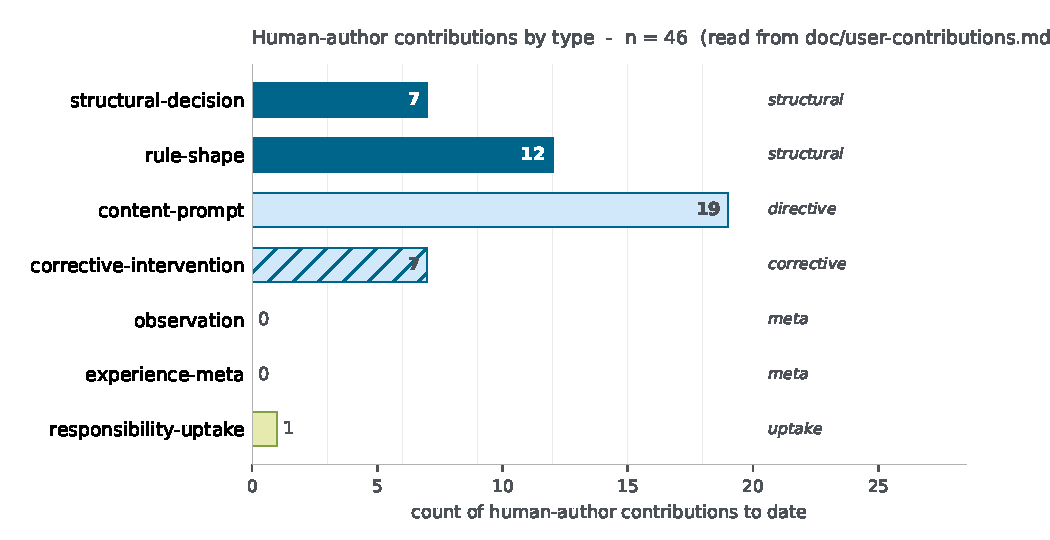
\includegraphics[width=0.92\linewidth]{figures/contribution-histogram.pdf}
\caption{Human-author contributions to the manuscript by type, read
from \texttt{doc/user-contributions.md}. Structural decisions and
rule-shape interventions are rare but high leverage; corrective
interventions are the catch-and-fix work; responsibility-uptake is
the leg of the contribution the AI structurally cannot share.
Regenerated on every build.}
\label{fig:contribution-histogram}
\end{figure}

A coupling rule sharpens the partition
(Figure~\ref{fig:coupling-rule}). The cooperation works as an
\emph{accelerator} when the model stays on the prose-craft side of
the partition --- drafting, cross-referencing, structuring ---
where its strength is interpolation within the manifold of prior
text~\cite{clark1998extended,hutchins1995cognition,clark2025extending}\todo[inline]{verify}.
It collapses toward a \emph{cultural blender} when the model is
allowed across into the abstracting layer, where its failure mode
is to smooth the unfamiliar into the nearest familiar
shape~\cite{anderson2024homogenization}\todo[inline]{verify}. The
diagnostic, recorded in the observations log: \emph{ask whether
the abstraction would have been thinkable without the model. If
yes, the model was an accelerator on that abstraction; if no, the
question genuinely opens.} F(AI)\textsuperscript{2}R is a case
where the answer is yes; the partition is what kept it that way.

\paragraph{Tokens out, tokens in.}
\LaTeX{}, prompt files, Turtle, and the build pipeline are
committed under permissive licences and remain machine-readable.
That is deliberate. A future agent compressing or extending this
work has the inputs needed to do so without laundering its
provenance through a binary PDF. The tokens go in; the tokens come
back out; the chain of attribution is what makes the round-trip
auditable.
